\documentclass{beamer}
\usepackage{luatexja}
\usepackage[mark=o]{dynkin-diagrams}
\usepackage{rank-2-roots}
\newtheorem{proposition}{Proposition}
\usetheme{metropolis}
\title{ディンキン図形を知る \\ (ルート系とディンキン図形)}
\author{宇佐見 公輔}
\date{2019年4月13日}
\begin{document}
\frame{\titlepage}

\begin{frame}
    \frametitle{ディンキン図形とは何か}

    「ルート系(root system)」と呼ばれる対象を図であらわしたものが
    「ディンキン図形(Dynkin diagram)」です。

    \begin{example}[ディンキン図形]
        \scalebox{3}{
            \dynkin{A}{3}
        }
        \scalebox{3}{
            \dynkin{C}{5}
        }
        \scalebox{3}{
            \dynkin{D}{4}
        }
        \scalebox{3}{
            \dynkin{E}{6}
        }
        \scalebox{3}{
            \dynkin{F}{4}
        }
        \scalebox{3}{
            \dynkin{G}{2}
        }
    \end{example}
\end{frame}

\begin{frame}
    \frametitle{ルート系とは何か}

    実ベクトル空間の部分集合で、ある特定の条件(これはもう少し後で述べます)を満たすものを
    「ルート系(root system)」と呼びます。

    \begin{example}[ルート系]
        \scalebox{2}{
            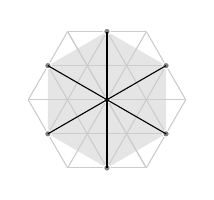
\begin{tikzpicture}
                \begin{rootSystem}{A}
                    \roots
                    \wt{0}{0}
                    \draw \weight{0}{0} -- \weight{1}{1};
                    \draw \weight{0}{0} -- \weight{-1}{-1};
                    \draw \weight{0}{0} -- \weight{1}{-2};
                    \draw \weight{0}{0} -- \weight{-1}{2};
                    \draw \weight{0}{0} -- \weight{2}{-1};
                    \draw \weight{0}{0} -- \weight{-2}{1};
                \end{rootSystem}
            \end{tikzpicture}
        }
        \scalebox{3}{
            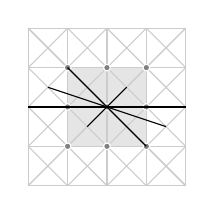
\begin{tikzpicture}
                \begin{rootSystem}{B}
                    \roots
                    \wt{0}{0}
                    \draw \weight{0}{0} -- \weight{0}{2};
                    \draw \weight{0}{0} -- \weight{0}{-2};
                    \draw \weight{0}{0} -- \weight{1}{0};
                    \draw \weight{0}{0} -- \weight{-1}{0};
                    \draw \weight{0}{0} -- \weight{1}{-2};
                    \draw \weight{0}{0} -- \weight{-1}{2};
                    \draw \weight{0}{0} -- \weight{2}{-2};
                    \draw \weight{0}{0} -- \weight{-2}{2};
                \end{rootSystem}
            \end{tikzpicture}
        }
    \end{example}
\end{frame}

\begin{frame}
    \frametitle{なぜルート系を考えるのか}

    ルート系は、リー代数(Lie algebra)を分類する研究の中であらわれました。

    \begin{itemize}
        \item 複素数体上の有限次元単純リー代数は、ルート分解という直和分解ができます。
        \item そこに出てくるルート(root)というベクトルの集合は、
              ある一定の性質を持っています。
        \item この性質をルート系の定義として、
              ルート系の分類をすることでリー代数の分類ができます。
    \end{itemize}

    その後、数学の様々な分野でルート系が登場することが知られるようになりました。
\end{frame}

\begin{frame}
    \frametitle{ルート系の定義の準備:鏡映}

    \(E\) を有限次元実ベクトル空間、
    \(v, w \in E\) の内積を \((v|w)\) とします。

    \begin{definition}[超平面]
        \(v \in E\) に対して
        \(P_v := \{ w \in E \mid (v|w) = 0 \} \)
        と定義し、\(v\) と直交する超平面(hyperplane)と呼びます。
    \end{definition}

    \begin{definition}[鏡映]
        \(v \in E\) と \(x \in E\) に対して、
        \[c(x,v) := \frac{2(x|v)}{(v|v)}\]
        と定義し、写像 \(\sigma_v : E \to E\) を以下で定義します。
        \[x \mapsto x - c(x,v) v\]
        \(\sigma_v\) を、超平面 \(P_v\) に関する鏡映(reflection)と呼びます。
    \end{definition}
\end{frame}

\begin{frame}
    \frametitle{ルート系の定義}

    \begin{definition}[ルート系]
        \(\Delta \subset E\) がルート系(root system)であるとは、以下を満たすことです。

        \begin{enumerate}
            \item \(\Delta \) は \(0\) を含まない有限集合で、\(E\) を張る。
            \item \(c \in \mathbb{R}\)、\(v \in \Delta \)、\(cv \in \Delta \)
                  のとき、\(c = \pm 1\) である。
            \item \(v \in \Delta \) のとき、\(\sigma_v(\Delta) = \Delta \) である。
            \item\label{cartanInt} \(v, w \in \Delta \) のとき、\(c(v,w) \in \mathbb{Z}\) である。
        \end{enumerate}

        また、ルート系の元をルート(root)と呼びます。
    \end{definition}

    条件 \ref{cartanInt} が少し分かりにくいですが、言葉でいえば、
    「\(v\) の鏡映 \(\sigma_v\) で \(w\) を移したときの差分が \(v\) の整数倍になる」
    という感じになります。
\end{frame}

\begin{frame}
    \frametitle{ルート系の例}

    \begin{example}[2次元空間のルート系]
        \begin{table}
            \begin{tabular}{cc}
                \scalebox{2}{
                    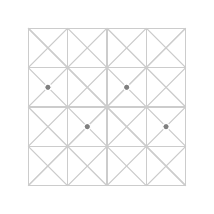
\begin{tikzpicture}
                        \begin{rootSystem}{B}
                            \wt{1}{0}
                            \wt{1}{-2}
                            \wt{-1}{2}
                            \wt{-1}{0}
                        \end{rootSystem}
                    \end{tikzpicture}
                } &
                \scalebox{2}{
                    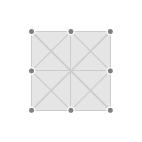
\begin{tikzpicture}
                        \begin{rootSystem}{B}
                            \roots
                        \end{rootSystem}
                    \end{tikzpicture}
                }   \\
                \scalebox{1.5}{
                    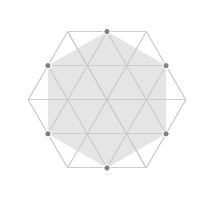
\begin{tikzpicture}
                        \begin{rootSystem}{A}
                            \roots
                        \end{rootSystem}
                    \end{tikzpicture}
                } &
                \scalebox{1.5}{
                    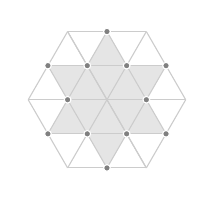
\begin{tikzpicture}
                        \begin{rootSystem}{G}
                            \roots
                        \end{rootSystem}
                    \end{tikzpicture}
                }
            \end{tabular}
        \end{table}
    \end{example}
\end{frame}

\begin{frame}
    \frametitle{2つのルートの関係}

    ベクトル \(v,w\) のなす角を \(\theta \) とします。

    \(c(v,w)\) の定義から \(c(v,w) c(w,v) = 4 \cos^2 \theta \) が導けます。

    ここで \(v, w\) をルートとし、それらが線型独立とすると、
    \(c(v,w) \in \mathbb{Z}\) から、
    \[
        c(v,w) c(w,v) = 0, 1, 2, 3
    \]
    となることが分かります。

    また、\(\theta \) のとりうる値は以下です。
    \[
        \frac{\pi}{2}, \frac{\pi}{3}, \frac{2\pi}{3},
        \frac{\pi}{4}, \frac{3\pi}{4}, \frac{\pi}{6}, \frac{5\pi}{6}
    \]
\end{frame}

\begin{frame}
    \frametitle{ルート系の底}

    ルート系には、基底のようなものが存在しています。

    \begin{proposition}[ルート系の底]
        \(\Delta \subset E\) をルート系とします。
        以下を満たす \(\Pi \subset \Delta \) が存在します。

        \begin{enumerate}
            \item \(\Pi \) は \(E\) の基底である。
            \item \(v \in \Delta \) を \(v = \sum_{e \in \Pi} c_e e\) とすると、
                  \(c_e\) は全て \(0\) 以上の整数、または全て \(0\) 以下の整数となる。
        \end{enumerate}

        \(\Pi \) を \(\Delta \) の底(base)と呼びます。
    \end{proposition}
\end{frame}

\begin{frame}
    \frametitle{ディンキン図形の定義}

    \begin{definition}[ディンキン図形]
        \(\Delta \) を \(n\) 次元空間のルート系、\(\Pi \) を \(\Delta \) の底とします。

        以下のように構成されるグラフを \(\Delta \) のディンキン図形(Dynkin diagram)と呼びます。

        \begin{enumerate}
            \item \(n\) 個のノードを持つ。各ノードは \(\Pi \) の元でラベルづけされる。
            \item ノードとノードを何本かの辺で結ぶ。
                  その本数は \(c(v,w) c(w,v)\) とする。
                  (したがって、0〜3本である)
            \item 辺で結ばれたノードについて、
                  \((v|v)\) と \((w|w)\) が異なる場合、
                  大きいほうのノードから小さいほうのノードへ矢印をつける。
        \end{enumerate}

        補足:\(c(v,w) c(w,v) = 1\) のときは \((v|v) = (w|w)\) であるため、
        矢印がつくのは辺が2本または3本のときとなります。
    \end{definition}
\end{frame}

\begin{frame}
    \frametitle{ディンキン図形の例}

    \begin{example}[2次元空間のルート系のディンキン図形]
        \begin{table}
            \begin{tabular}{cccc}
                \scalebox{1.5}{
                    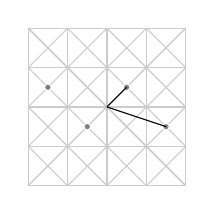
\begin{tikzpicture}
                        \begin{rootSystem}{B}
                            \wt{1}{0}
                            \wt{1}{-2}
                            \wt{-1}{2}
                            \wt{-1}{0}
                            \draw \weight{0}{0} -- \weight{1}{0};
                            \draw \weight{0}{0} -- \weight{-1}{2};
                        \end{rootSystem}
                    \end{tikzpicture}
                } &
                \scalebox{2}{
                    \dynkin{A}{1}
                    \dynkin{A}{1}
                } &
                \scalebox{1.5}{
                    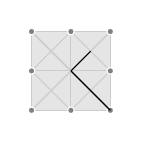
\begin{tikzpicture}
                        \begin{rootSystem}{B}
                            \roots
                            \draw \weight{0}{0} -- \weight{1}{0};
                            \draw \weight{0}{0} -- \weight{-2}{2};
                        \end{rootSystem}
                    \end{tikzpicture}
                } &
                \scalebox{2}{
                    \dynkin{B}{2}
                }   \\
                \scalebox{1.2}{
                    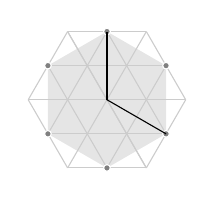
\begin{tikzpicture}
                        \begin{rootSystem}{A}
                            \roots
                            \draw \weight{0}{0} -- \weight{2}{-1};
                            \draw \weight{0}{0} -- \weight{-1}{2};
                        \end{rootSystem}
                    \end{tikzpicture}
                } &
                \scalebox{2}{
                    \dynkin{A}{2}
                } &
                \scalebox{1.2}{
                    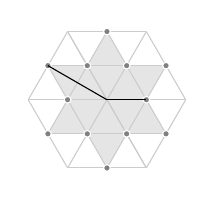
\begin{tikzpicture}
                        \begin{rootSystem}{G}
                            \roots
                            \draw \weight{0}{0} -- \weight{1}{0};
                            \draw \weight{0}{0} -- \weight{-3}{1};
                        \end{rootSystem}
                    \end{tikzpicture}
                } &
                \scalebox{2}{
                    \dynkin{G}{2}
                }
            \end{tabular}
        \end{table}
    \end{example}
\end{frame}

\begin{frame}
    \frametitle{なぜディンキン図形を考えるのか}

    ルート系の性質をディンキン図形の性質に置きかえると、簡単な性質になります。
    例えば、以下のような性質が導けます。

    \begin{itemize}
        \item ループを持たない。
        \item 分岐は多くともひとつしかない。
        \item ひとつのノードから出る辺は3本以内である。
    \end{itemize}

    また、分岐がある場合にそれぞれの分岐はどのくらいの長さが可能か、
    といった議論もできます。

    これらを使って可能なディンキン図形を分類することで、
    ルート系の分類ができます。
\end{frame}

\begin{frame}
    \frametitle{ディンキン図形の分類}

    \begin{theorem}[ディンキン図形の分類]
        ディンキン図形は以下のいずれかと一致する。
        また、以下のディンキン図形に対応するルート系が存在する。

        \begin{itemize}
            \item \(A_n\) (\(n \geq 1\))
            \item \(B_n\) (\(n \geq 2\))
            \item \(C_n\) (\(n \geq 3\))
            \item \(D_n\) (\(n \geq 4\))
            \item \(E_n\) (\(n = 6,7,8\))
            \item \(F_4\)
            \item \(G_2\)
        \end{itemize}
    \end{theorem}

    具体的な図は次ページ以降で。
\end{frame}

\begin{frame}
    \frametitle{ディンキン図形:古典型}

    \begin{table}
        \begin{tabular}{cc}
            \(A_n\) &
            \scalebox{3}{
                \dynkin{A}{}
            } \\
            \(B_n\) &
            \scalebox{3}{
                \dynkin{B}{}
            } \\
            \(C_n\) &
            \scalebox{3}{
                \dynkin{C}{}
            } \\
            \(D_n\) &
            \scalebox{3}{
                \dynkin{D}{}
            }
        \end{tabular}
    \end{table}
\end{frame}

\begin{frame}
    \frametitle{ディンキン図形:例外型}

    \begin{table}
        \begin{tabular}{cc}
            \(E_6\) &
            \scalebox{2.5}{
                \dynkin{E}{6}
            } \\
            \(E_7\) &
            \scalebox{2.5}{
                \dynkin{E}{7}
            } \\
            \(E_8\) &
            \scalebox{2.5}{
                \dynkin{E}{8}
            } \\
            \(F_4\) &
            \scalebox{2.5}{
                \dynkin{F}{4}
            } \\
            \(G_2\) &
            \scalebox{2.5}{
                \dynkin{G}{2}
            }
        \end{tabular}
    \end{table}
\end{frame}

\begin{frame}
    \frametitle{ルート系とディンキン図形の面白さ}
    
    個人的に思う、ルート系とディンキン図形の面白さは以下のようなところです。

    \begin{itemize}
        \item ルート系の性質が簡単なグラフ上の性質に置き換わる
        \item 分類結果が多すぎず少なすぎず、ちょうどいいくらいの種類
        \item 例外型に感じられるロマン
        \item いろいろな分野に顔を出す意外性
    \end{itemize}

    決して難しい理論ではないので、ぜひ触れてみてください。

    また、拡大ディンキン図形など、類似の図形もいろいろあるので、
    調べてみると面白いかと思います。
\end{frame}

\end{document}
